\chapter{Radio communication with the nanosatellites - state of the art}

\section{Subsystem review}
There are number of commercially available solutions and subsystems. Usually they are divided into subsystems, allowing user to mix different suppliers depending on the requirements, assuring they are compatible.

\subsection{Cubesat commmunication diagram}
Typical Low Earth Orbit satellite communication systems is shown in the figure \ref{comm_diagram}.

\begin{figure}
    \centering
    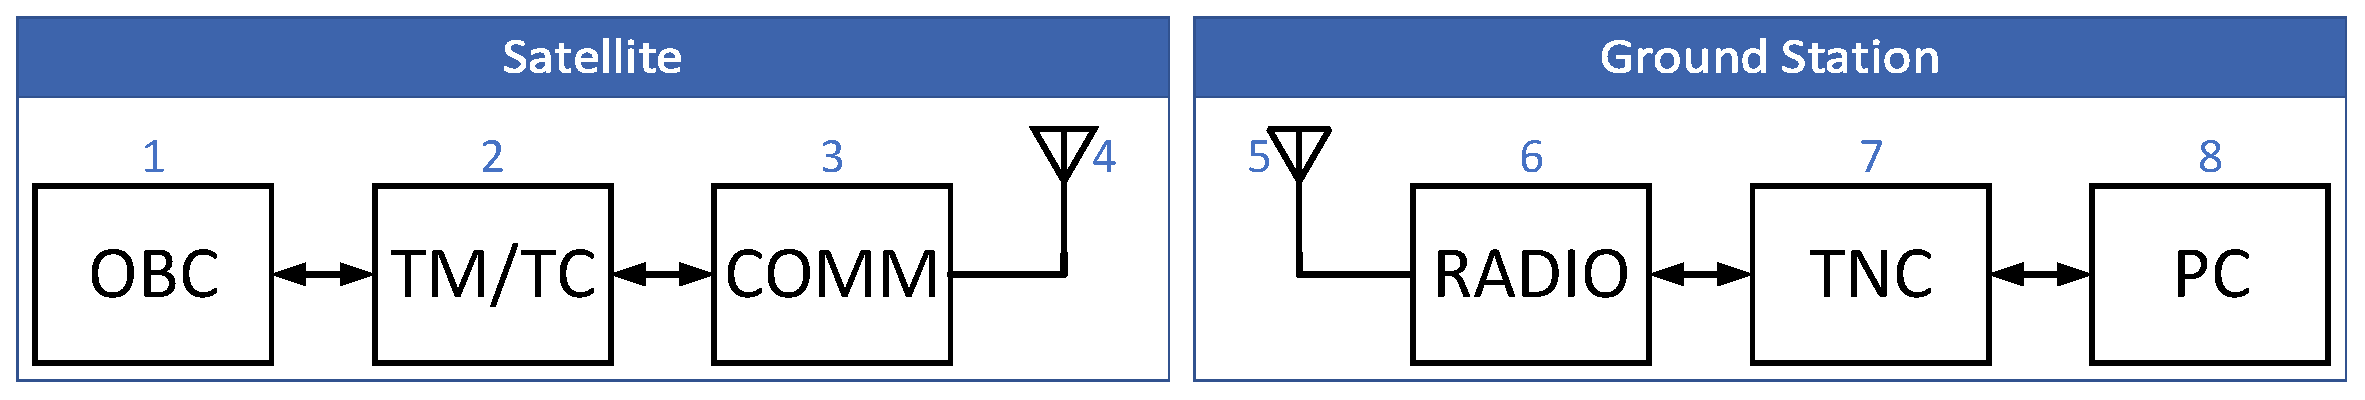
\includegraphics[width=0.7\paperwidth]{img/2/comm_diagram.eps}
    \caption{General communication system diagram}
    \label{comm_diagram}
\end{figure}

It consists of:
\begin{enumerate}
    \item On-Board Computer - controls the satellite, generates data and receives telecommands,
    \item Telemetry/Telecommand generator - translates between packets and baseband signal (modulator and demodulator),
    \item COMM - communications module, performs up/down conversion, amplification and antenna matching, usually on smaller missions it is integrated with TMTC on one module,
    \item Satellite antenna(s), typically omnidirectional to provide coverage during random satellite tumbling
    \item Ground station antenna(s), directional to maximize gain of the radio link,
    \item RADIO - radio system, typically a low noise amplifier with up/down converter and modulator, converts radio frequencies to baseband signals,
    \item Terimnal Network Controller - translates between packets and baseband signal, can be done as a separate device or in software in the PC,
    \item PC - a computer, which operator of the satellite uses to generate and receive data packets.
\end{enumerate}

\subsection{Cubesat antennas}
Cubesat dimensions are strict and defined in the CubeSat Design Specification \cite{cubesat_spec} as \si{100}x\si{100}~mm square \ref{CubeSat_max_dim}. This poses a requirement of antenna unfolding for antennas larger than side width. Usually this is required for all sub-GHz band, such as considered VHF and UHF bands. Higher bands, such an S-band, usually use patch antennas mounted on the wall.

\begin{figure}
    \centering
    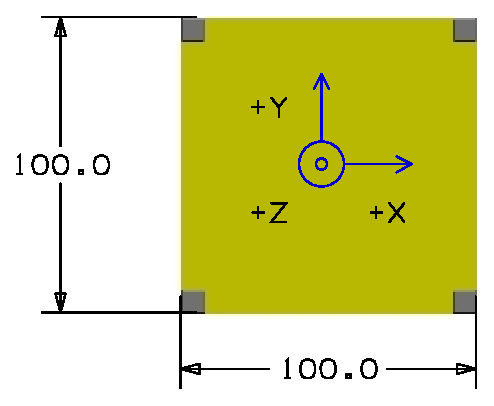
\includegraphics[width=0.5\paperwidth]{img/2/cubesat_dimensions.eps}
    \caption{CubeSat maximum dimensions, top view. Source \cite{cubesat_spec}.}.
    \label{CubeSat_max_dim}
\end{figure}

Antennas are usually unfolded by the spring action of the antennas itself and they are released by the on-board computer (by the thermal knife). Three typical antenna deployment systems are shown in the figures \ref{stiff_antenna_pic}, \ref{m_cubed}, \ref{isis_dipole_antenna}.

Typical unidirectional VHF/UHF antennas are dipoles, monopoles or turnstille. Selecting one depends on the mission requirements and link budget. Turnstille antenna, providing best link budget and circular polarization require that radiation elements are mounted on two sides of the CubeSat. Dipole option uses two elements is not as dependent on the ground reference (main structure) as the monopole antenna.

\begin{figure}
    \centering
    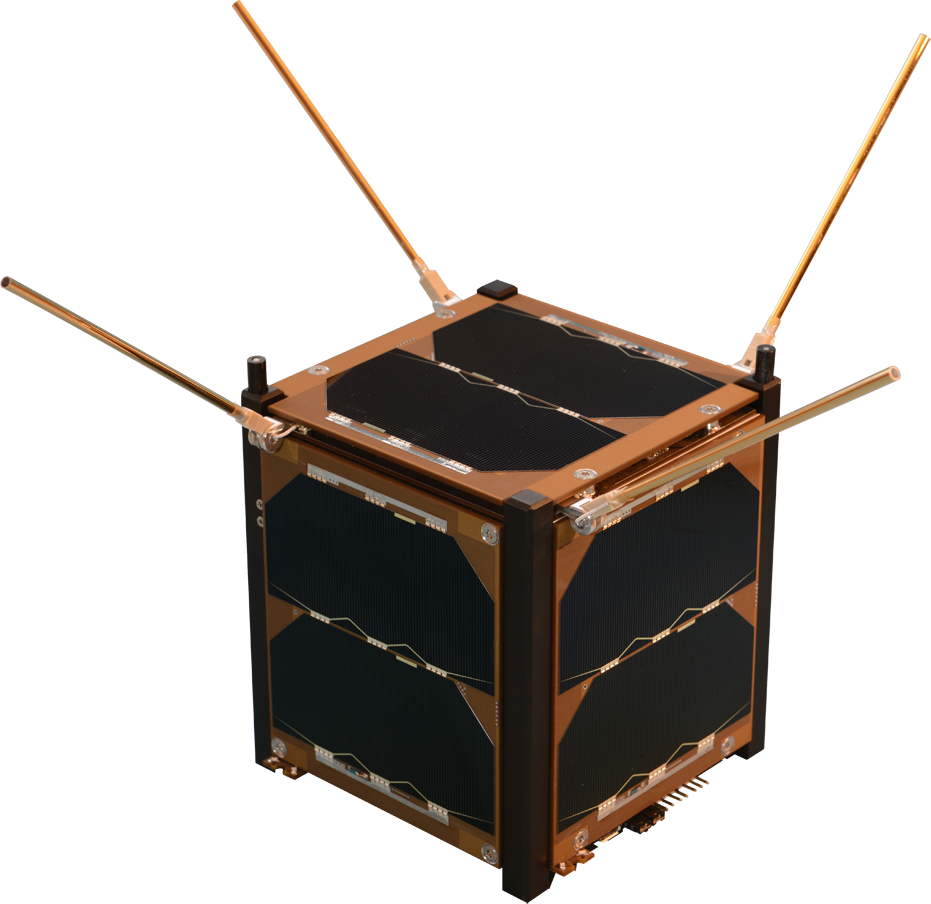
\includegraphics[width=0.5\paperwidth]{img/2/antenna_stiff.png}
    \caption{Deployed stiff antenna. In the stowed configuration they are along the solar panels. Source \cite{stiff_antenna_paper}.}.
    \label{stiff_antenna_pic}
\end{figure}

\begin{figure}
    \centering
    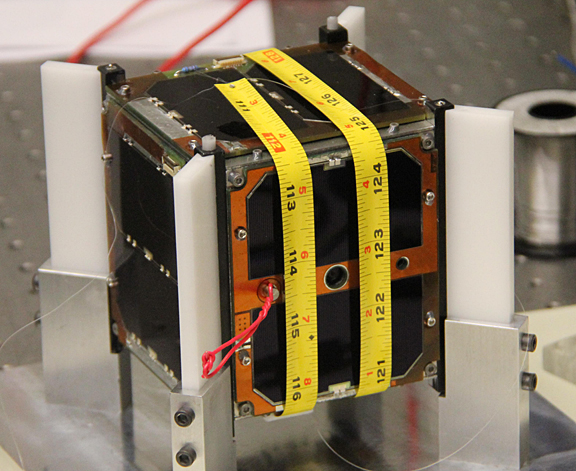
\includegraphics[width=0.5\paperwidth]{img/2/m-cubed.jpg}
    \caption{Tape measure antenna in the stowed configuration. Flat spring action forces antenna to deploy itself after its release. Source \cite{m_cubed}.}.
    \label{m_cubed}
\end{figure}

\begin{figure}
    \centering
    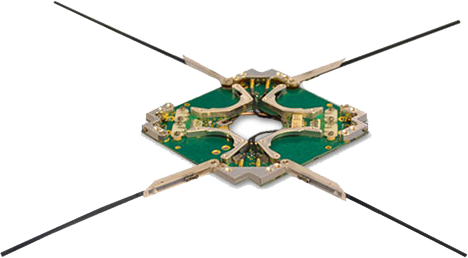
\includegraphics[width=0.5\paperwidth]{img/2/isis_dipole.png}
    \caption{Flat spring antennas rolled inside the CubeSat square. Released by the thermal knife burning the lock of the antenna doors. Source \cite{isis_dipole_antenna}.}.
    \label{isis_dipole_antenna}
\end{figure}

\subsection{Ground station antennas}
Space communication antennas require very large gain due to the distance between the stations and the omnidirectivity of the CubeSat antennas. Transmit power of the satellite is usually rather low (\SI{1}{\watt} or less).

Most of the designs use Yagi-Uda antennas, in circular polarization (cross-yagi with phasing). They are typically 9-11 elements long for VHF and 17-19 elements for UHF. Yagi-Uda antennas can be also phased as an array of antennas (1x2, 2x2 configuration etc.) improving gain and directivity. This however requires the antenna mast to withstand the size and weight of the system. Required power gain is dependent on the mission itself and the reliability of the link. Random tumbling and CubeSat antennas with dips in the radiation pattern (as monopole and dipole) require more directivity and power gain than attitude-controlled satellites. Direcitivity of the antenna also affects antenna noise temperature.

Depending on the mission, one, two or more antennas can be required due to the number of bands used. 

Due to the directivity of the antennas, their half-power beam width is around \si{2}-\SI{10}{\degree}. Therefore another required element of the ground station is the antenna rotator, which has to support the required weight, size and the location of the ground station.

In the figure \ref{isis_gs} the commercially available ISIS VHF/UHF ground station is shown, which employs two cross-yagi antennas (VHF, UHF), antenna mast and rotator and rotator controller.

\begin{figure}
    \centering
    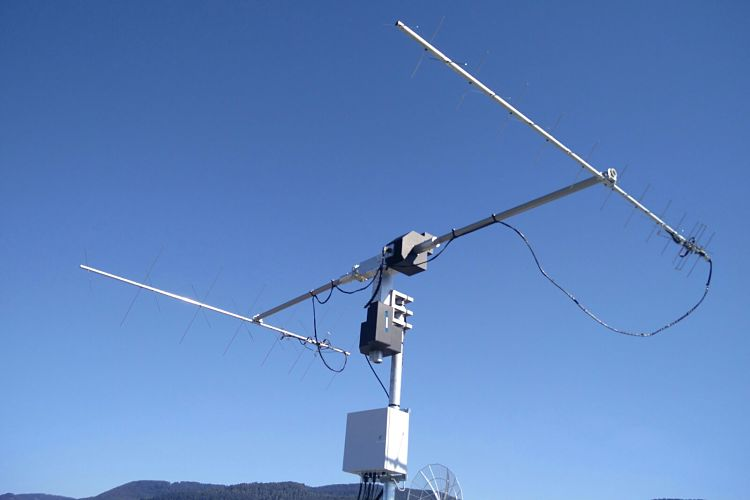
\includegraphics[width=0.5\paperwidth]{img/2/isis_gs.jpg}
    \caption{ISIS Ground Station. Source \cite{isis_gs}.}.
    \label{isis_gs}
\end{figure}

\subsection{Satellite communication subsystem}
Communication subsystem of the satellite is responsible of transmitting and receiving radio signals, modulating/demodulating them and providing data link for the On Board Computer. It has to be compatible with selected mechanical configuration, available data interfaces and the antennas to be installed. Most of the designs use custom design radio systems, using heterodyne receivers/transmitters (Fig. \ref{clyde_comm}), however there are an Software-Defined Radio systems, such as Gomspace SDR Platform \ref{gomspace_comm}.

\begin{minipage}{\linewidth}
    \centering
    \begin{minipage}{0.45\linewidth}
        \begin{figure}[H]
            \centering
            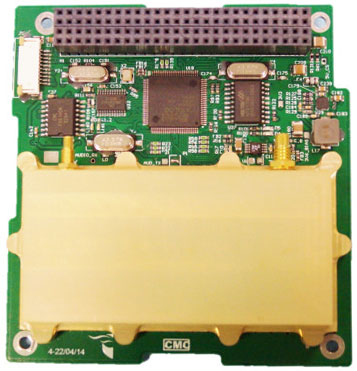
\includegraphics[width=0.32\paperwidth]{img/2/clyde_comm.jpg}
            \caption{CPUT UTRX from Clyde Space. Source: \cite{clyde_comm}}
            \label{clyde_comm}
        \end{figure}
    \end{minipage}
    \hspace{0.05\linewidth}
    \begin{minipage}{0.45\linewidth}
        \begin{figure}[H]
            \centering
            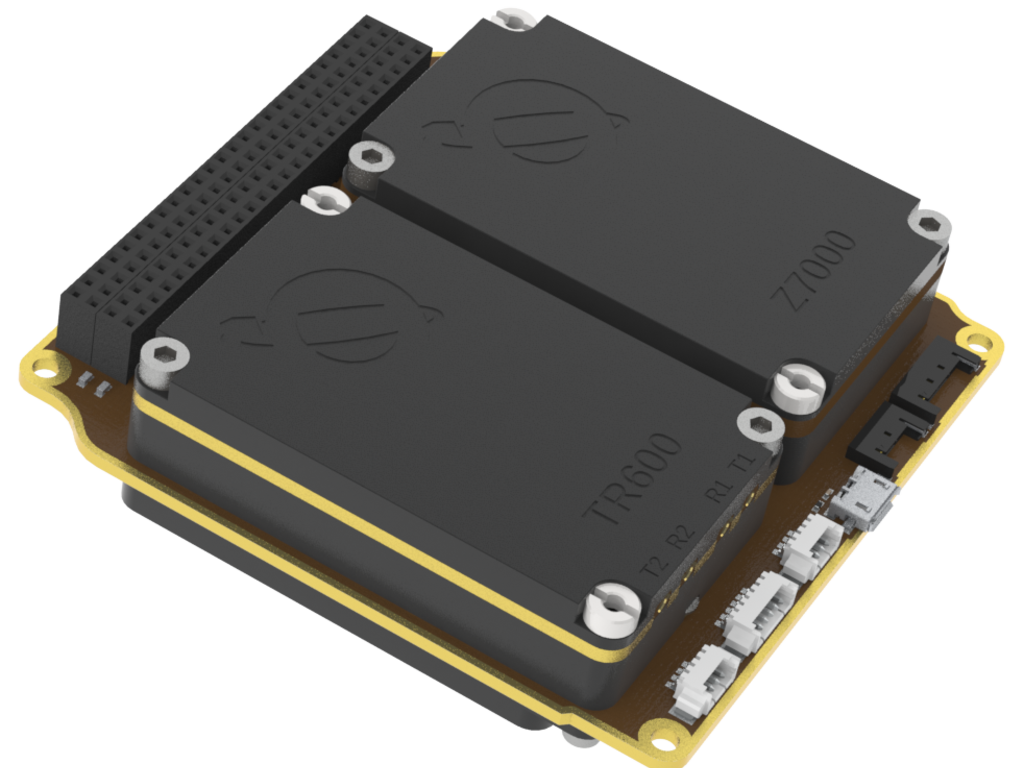
\includegraphics[width=0.35\paperwidth]{img/2/gomspace_sdr.png}
            \caption{Space qualified Software Defined Radio (SDR) Platform. Source: \cite{gomspace_comm}}
            \label{gomspace_comm}
        \end{figure}
    \end{minipage}
\end{minipage}


\subsection{Ground segment communication subsystem}
\subsubsection{Transmitter}
Due to the typically lower sensitivity and omnidirectional antenna on the satellite the uplink EIRP has to be very large, requiring not only directional antennas but also high output power (\si{100}-\SI{1500}{\watt}).
Depending on the modulation required, relatively cheap radio amateur transceivers can be used to modulate and amplify transmit signals, such as ICOM 910H or KENWOOD TS-2000 E (Fig. \ref{kenwood_ts2000}). As those types of radios were designed to transmit speech (bandwidth up to about \SI{10}{\kHz}) they can be used only to transmit signals which are FM, AM or SSB modulated. For other modulation and/or bandwidth the radio signal has to be generated by other type of radio (integrated or software-defined) and power amplifier.

Depending on the required output power, high-power amplifier can be used to further increase output power up to several kilo-watts. 

\begin{minipage}{\linewidth}
    \centering
    \begin{minipage}{0.45\linewidth}
        \begin{figure}[H]
            \centering
            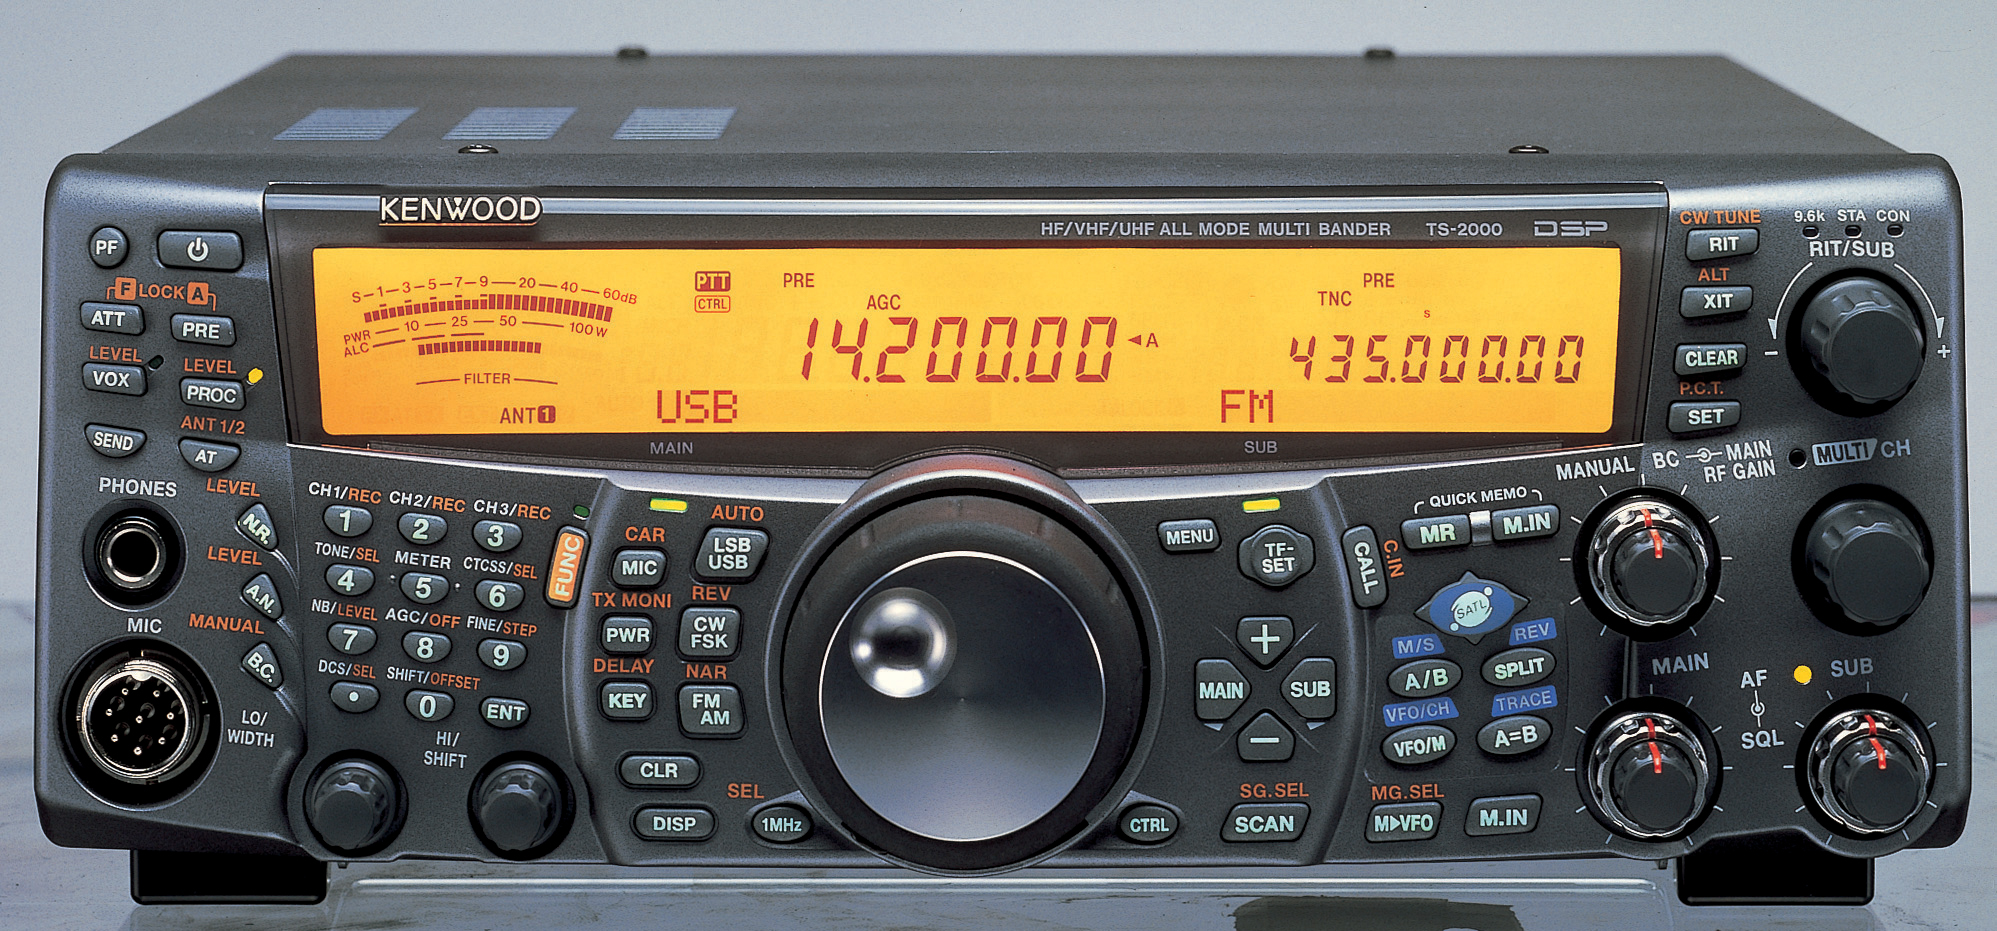
\includegraphics[width=0.35\paperwidth]{img/2/kenwood_ts2000.jpg}
            \caption{KENWOOD TS-2000 E all mode transceiver. Source: \cite{kenwood_ts2000}}
            \label{kenwood_ts2000}
        \end{figure}
    \end{minipage}
    \hspace{0.05\linewidth}
    \begin{minipage}{0.45\linewidth}
        \begin{figure}[H]
            \centering
            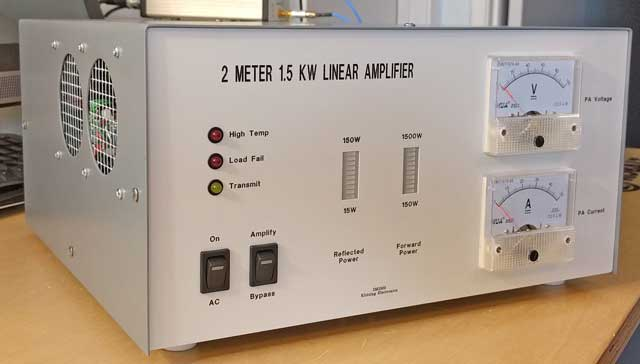
\includegraphics[width=0.35\paperwidth]{img/2/vhf_1500w_pa.jpg}
            \caption{\SI{1500}{\watt} VHF power amplifier. Source: \cite{vhf_1500w_pa}}
            \label{vhf_1500w_pa}
        \end{figure}
    \end{minipage}
\end{minipage}

\subsubsection{Receiver}
The receiver on the ground has to complement the space segment. Due to relatively low transmit power on the satellite, the receiver sensitivity should be very high. Additionally, receiver intermodulation performance should withstand possible blocking signals which are present on the ground.

To increase the sensitivity, Low Noise Amplifier has to be installed close to the antenna, such as LNA SSB-70 for UHF band (Fig. \ref{ssb_lna70}), which has Noise Figure of about \SI{0.35}{\dB}. Intermodulation and blocking is provided at the first stage by placing low-loss filter before the LNA, such as Cavity filters (Fig. \ref{cavity_uhf}).

\begin{minipage}{\linewidth}
    \centering
    \begin{minipage}{0.45\linewidth}
        \begin{figure}[H]
            \centering
            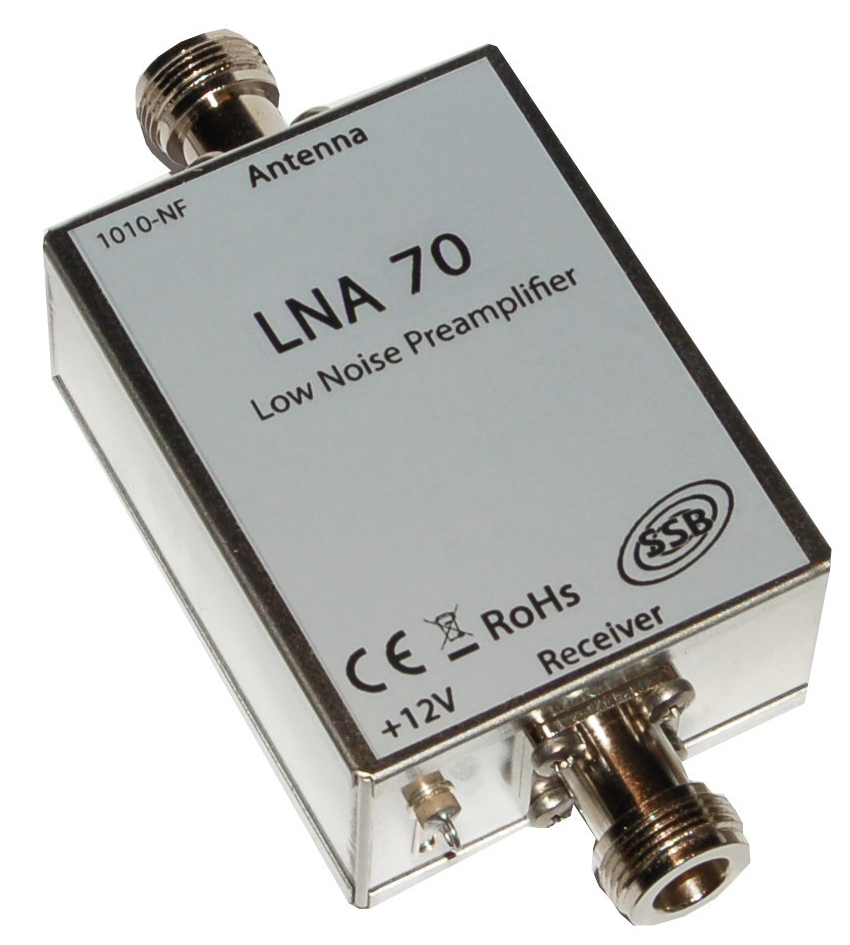
\includegraphics[width=0.3\paperwidth]{img/2/ssb_lna70.jpg}
            \caption{LNA SSB-70 Low Noise Amplifier for UHF band. Source: \cite{ssb_lna70}}
            \label{ssb_lna70}
        \end{figure}
    \end{minipage}
    \hspace{0.05\linewidth}
    \begin{minipage}{0.45\linewidth}
        \begin{figure}[H]
            \centering
            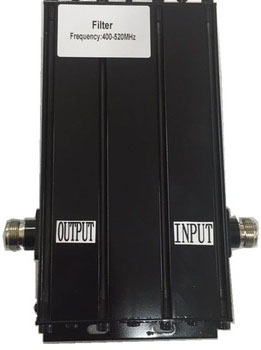
\includegraphics[width=10cm]{img/2/cavity_uhf.jpg}
            \caption{LBQ-450 3-cavity UHF bandpass filter. Source: \cite{cavity_uhf}}
            \label{cavity_uhf}
        \end{figure}
    \end{minipage}
\end{minipage}


Radio signal, pre-amplified by the low-noise amplifier is down-converted to the baseband and de-modulated. This can be performed by the integrated radio transceiver (same as the transmitter, this emposes the same modulation constraints as for the transmitter) or by the software-defined radio, such as an NI-USRP 2901 (Fig. \ref{ni_2901}) or FUNCube Dongle Pro+ (which was specifically designed for the FUNCube CubeSat - Fig. \ref{funcube}).

\begin{minipage}{\linewidth}
    \centering
    \begin{minipage}{0.45\linewidth}
        \begin{figure}[H]
            \centering
            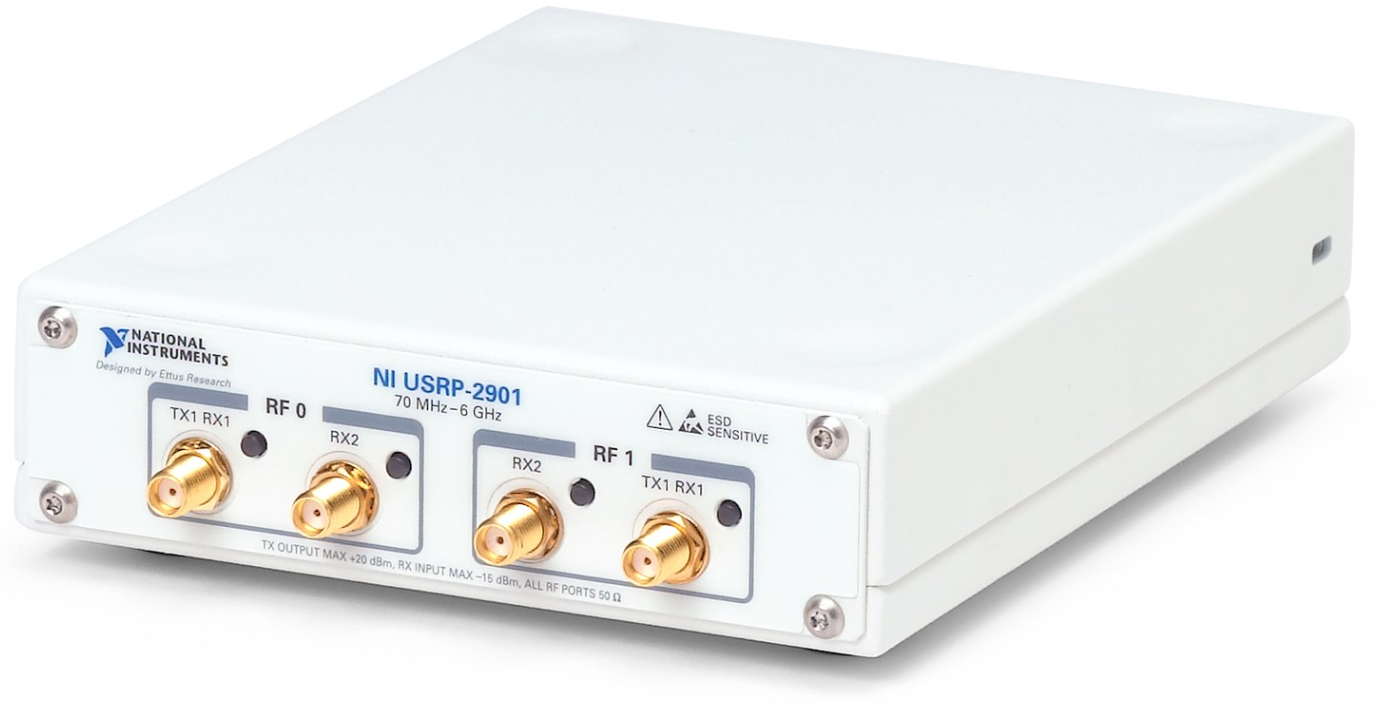
\includegraphics[width=0.3\paperwidth]{img/2/ni_2901.png}
            \caption{USRP-2901 Software Defined Radio Device. Source: \cite{ni_2901}}
            \label{ni_2901}
        \end{figure}
    \end{minipage}
    \hspace{0.05\linewidth}
    \begin{minipage}{0.45\linewidth}
        \begin{figure}[H]
            \centering
            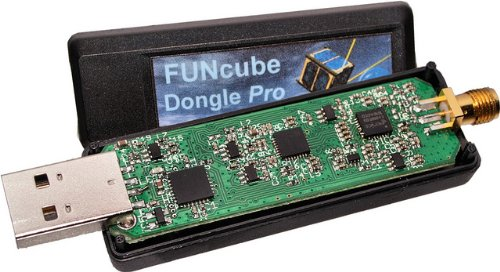
\includegraphics[width=0.3\paperwidth]{img/2/funcube.jpg}
            \caption{FUNcube Dongle Pro+. Source: \cite{funcube}}
            \label{funcube}
        \end{figure}
    \end{minipage}
\end{minipage}

After down-conversion baseband signal has to be de-modulated, which is done by the Terminal Network Controller. This can be implemeneted as a custom hardware solution (analog-to-digital converter and custom digital signal processor, for example TNC-X shown in the figure \ref{tncx}) or by pure software. Software solution has more flexibility but require a PC to perform signal processing, as is the only option for software-defined radio. One of the available TNC software using audio card is the Direwolf \cite{direwolf}.

\begin{figure}
    \centering
    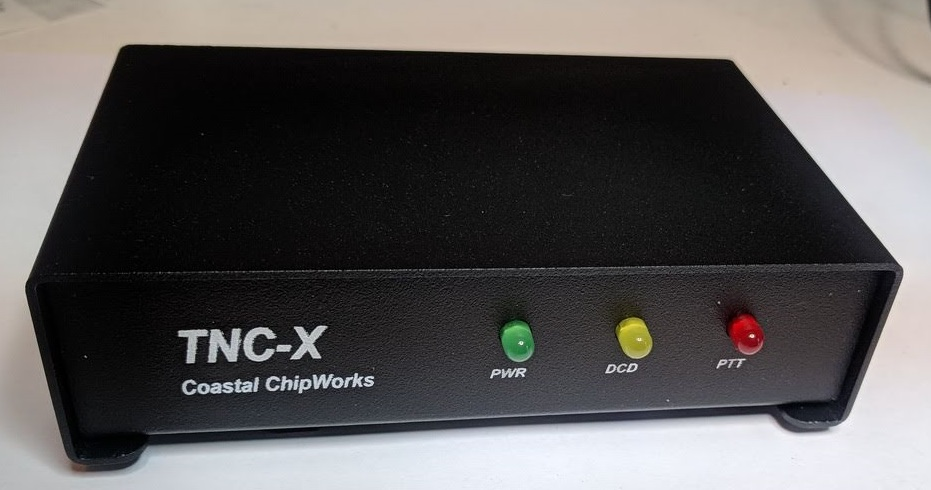
\includegraphics[width=0.3\paperwidth]{img/2/tncx.jpg}
    \caption{Terminal Network Controller TNC-X. Source: \cite{tncx}}
    \label{tncx}
\end{figure}



\section{Similar missions and designs}
In this section, three already flown satellite missions are described: PW-Sat, SwissCube and MOVE-I. 
\subsection{PW-Sat}
First polish satellite, PW-Sat, was launched in year \si{2012}. It was build on Warsaw Univeristy of Technology, with Space Research Centre PAS support. 

PW-Sat used ISIS TRXUV on-board communication module, with two (UHF uplink + VHF downlink) dipoles. Used modulations were AFSK \SI{1200}{\bps}. Radio transmit output power was \SI{30}{\dBm}. 
Ground station was built on Nicolaus Copernicus Astronomical Center in Warsaw, using \si{4}, \si{9}~element synphase cross-yagi VHF antennas for downlink and \si{4}, \si{19}~element synphase cross-yagi UHF antennas for uplink. Peak output power for uplink was \SI{100}{\watt} from the ICOM 910H transceiver.

PW-Sat and its ground station antennas are shown in the figures \ref{PW-Sat1_pic} and \ref{CAMK_pic}.

\begin{minipage}{\linewidth}
    \centering
    \begin{minipage}{0.45\linewidth}
        \begin{figure}[H]
            \centering
            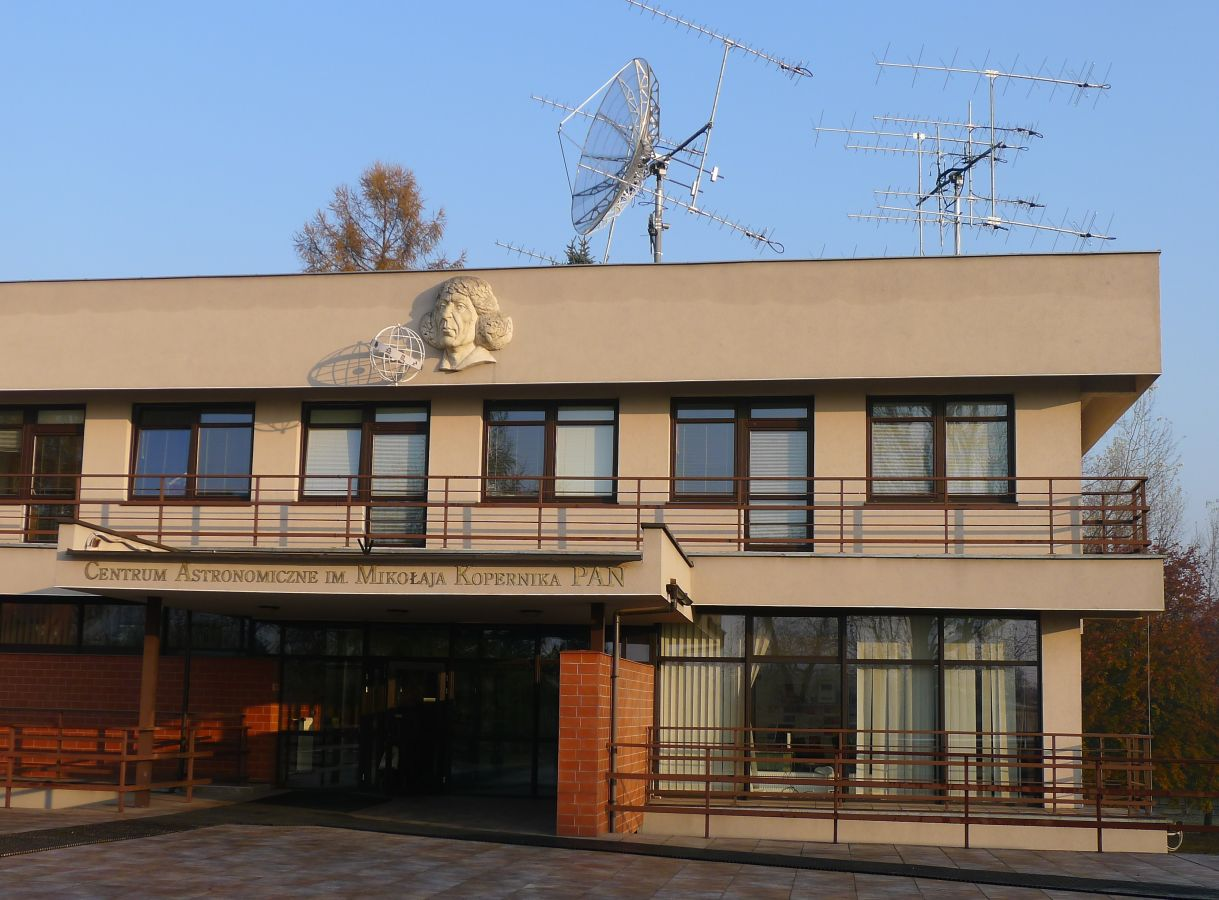
\includegraphics[width=0.32\paperwidth]{img/2/camk_pic.jpg}
            \caption{Nicolaus Copernicus Astronomical Center in Warsaw. PW-Sat antennas on the right. Source: \cite{camk_pic}}
            \label{CAMK_pic}
        \end{figure}
    \end{minipage}
    \hspace{0.05\linewidth}
    \begin{minipage}{0.45\linewidth}
        \begin{figure}[H]
            \centering
            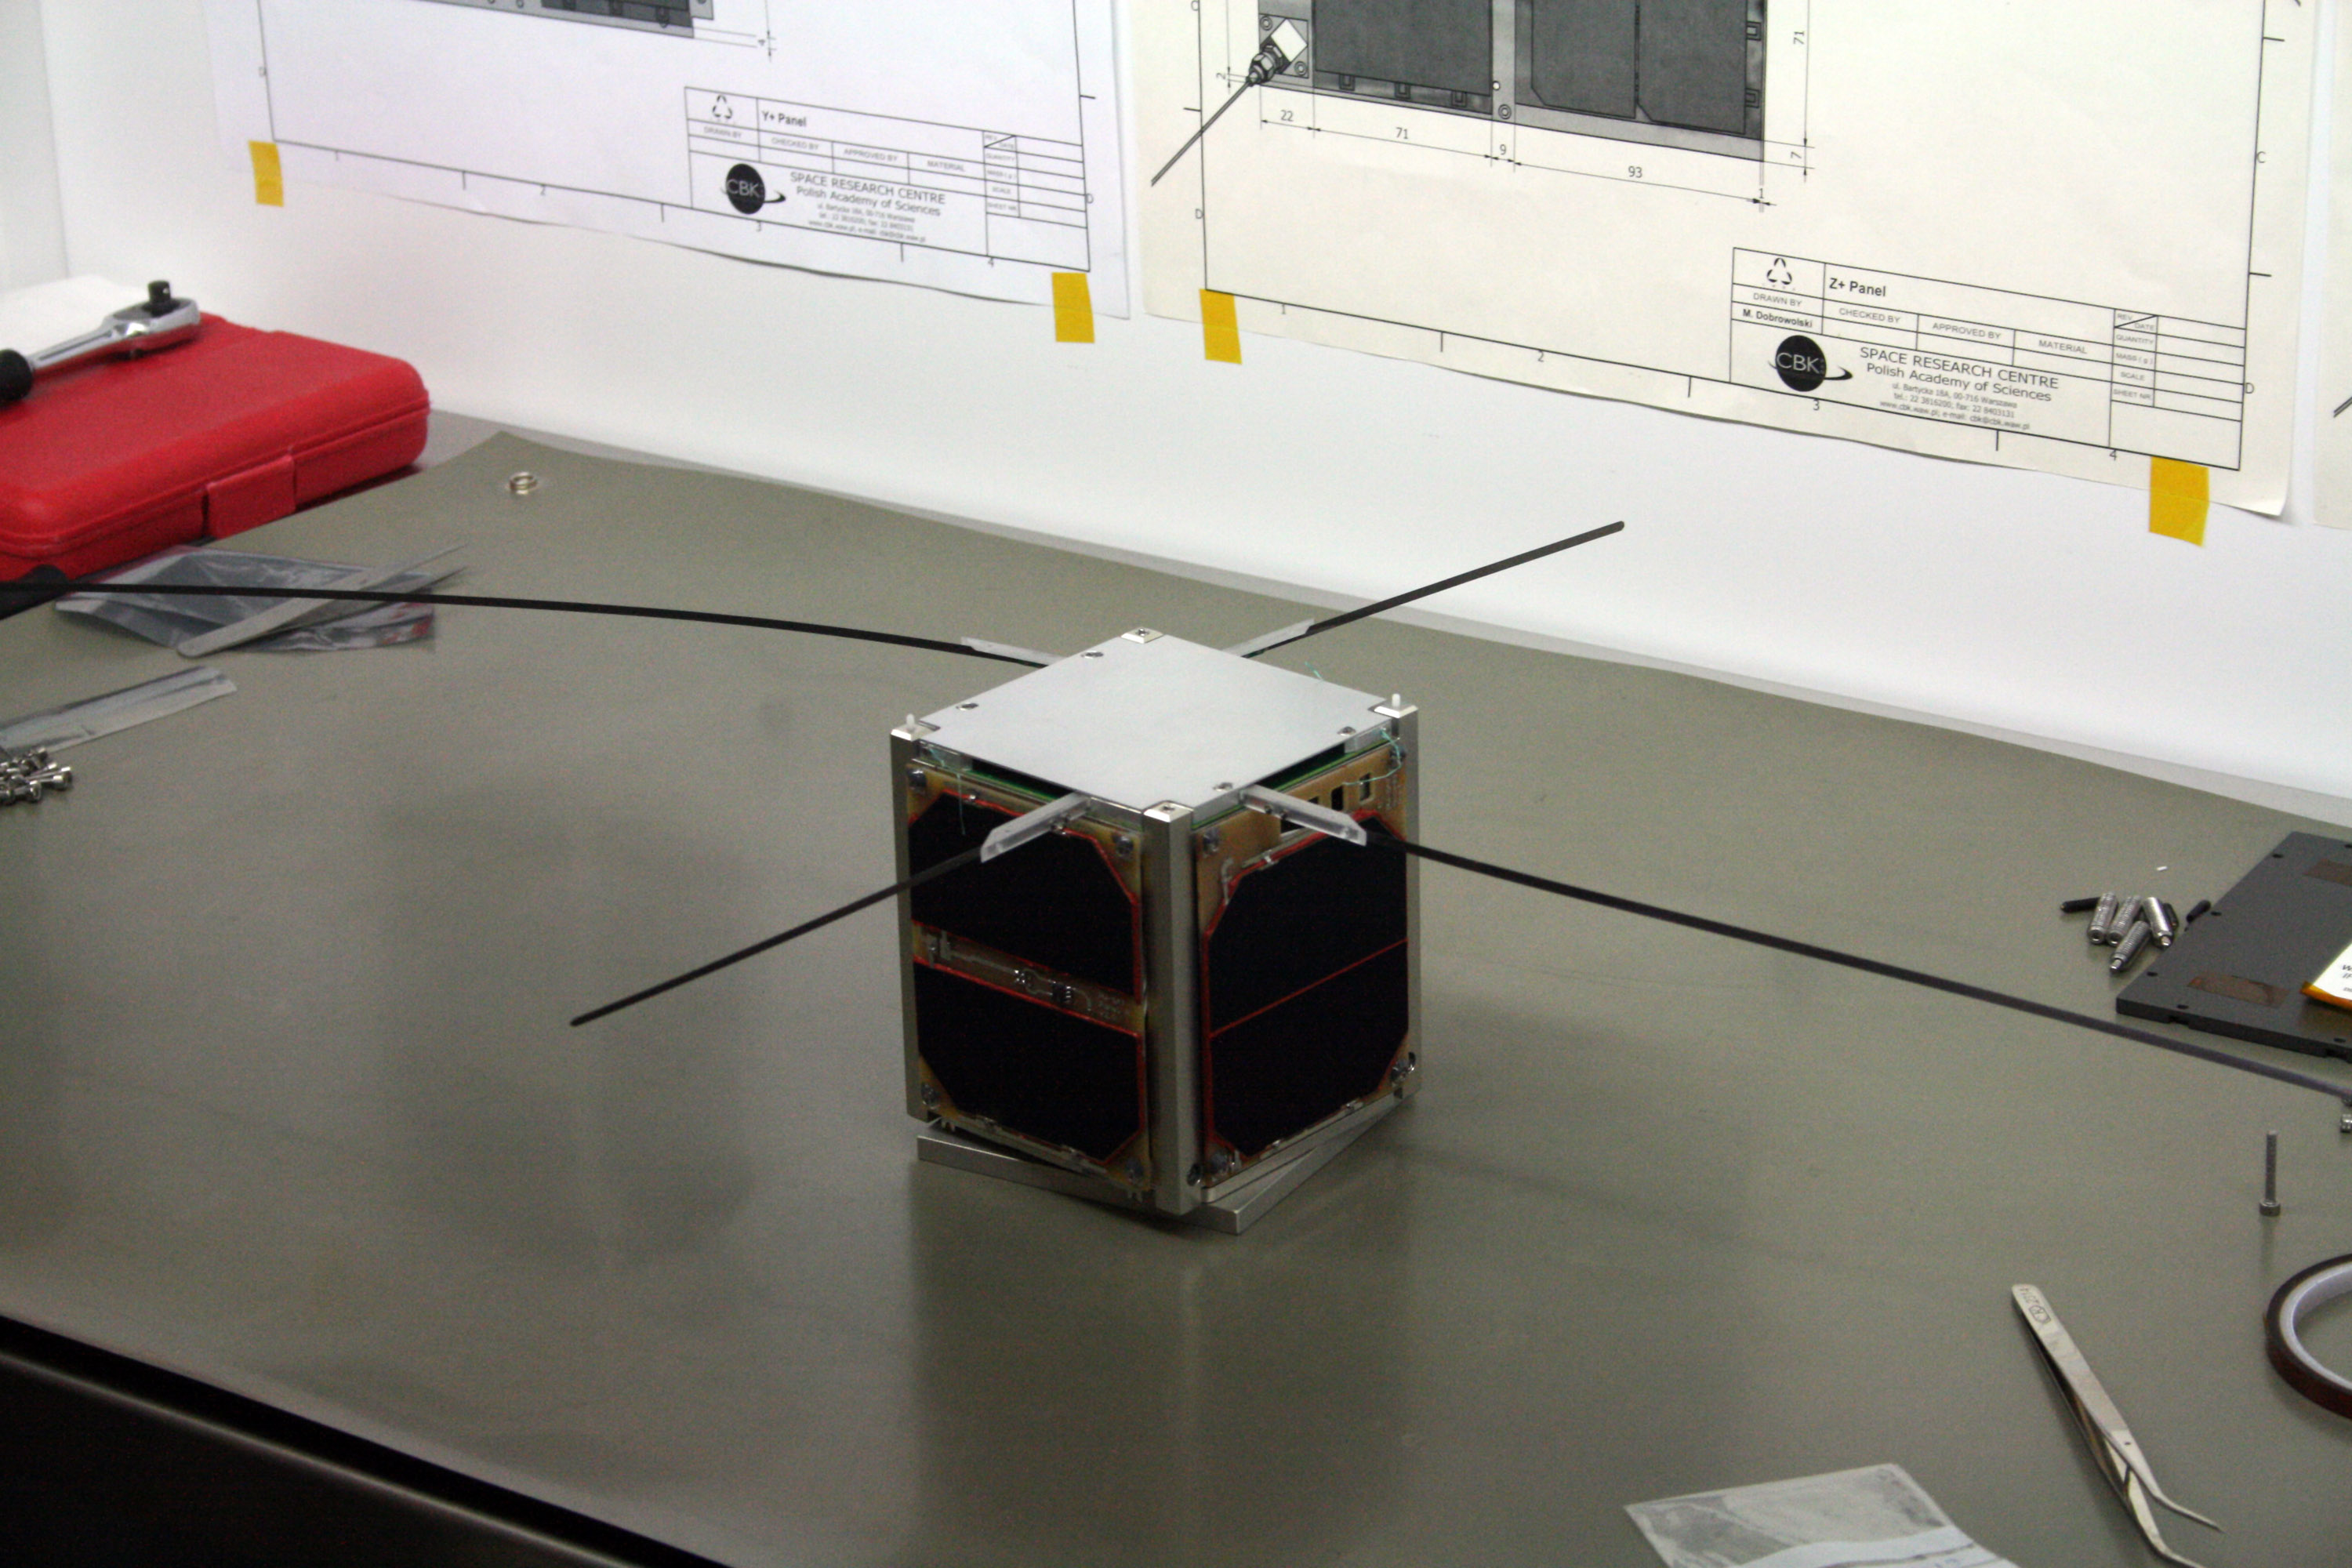
\includegraphics[width=0.32\paperwidth]{img/2/pw-sat1.jpg}
            \caption{PW-Sat1. Source: \cite{pwsat1_website_ska}}
            \label{PW-Sat1_pic}
        \end{figure}
    \end{minipage}
\end{minipage}

\subsection{SwissCube}
SwissCube is the first Swiss satellite, launched in 2009. SwissCube is 1U CubeSat, with two monopole antennas (VHF + UHF) rolled on one panel and deployed on-orbit. Housekeeping data downlink (basic telemetry) use constant \si{10}~WPM Morse code, with \SI{120}{\milli\watt} output power at \SI{437}{\MHz}. Full operational data is sent using \SI{1}{\watt} FSK modulation, \SI{1200}{\bps}. Uplink use FM-modulated AFSK signal on VHF. 

SwissCube use two Ground Stations, one at EPFL, and one at HE-Fribourg. The HE-Fribourg ground station uplink has \SI{11.4}{\dBi} of antenna-gain (one crossed \si{9}-element yagi). The downlink has \SI{14.5}{\dBi} of antenna gain (one crossed \si{17}-element yagi). The second ground station is located at EPFL in Lausanne. The performances of the EPFL ground station are slightly higher than the performances of the Fribourg ground station as there are \si{4} \si{70}-cm yagi antennas in reception (\SI{20.4}{\dBi} gain) and \si{2} \si{2}-m yagi antennas in emission (\SI{13}{\dBi} gain). \cite{swisscube_groundstation}

\begin{minipage}{\linewidth}
    \centering
    \begin{minipage}{0.45\linewidth}
        \begin{figure}[H]
            \centering
            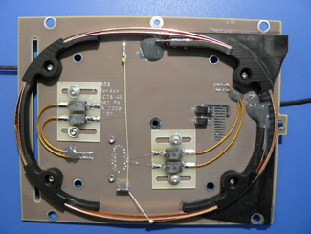
\includegraphics[width=0.32\paperwidth]{img/2/swisscube_stowed.png}
            \caption{SwissCube antennas in the stowed configuration. Source: \cite{swisscube_stowed}}
            \label{swisscube_stowed}
        \end{figure}
    \end{minipage}
    \hspace{0.05\linewidth}
    \begin{minipage}{0.45\linewidth}
        \begin{figure}[H]
            \centering
            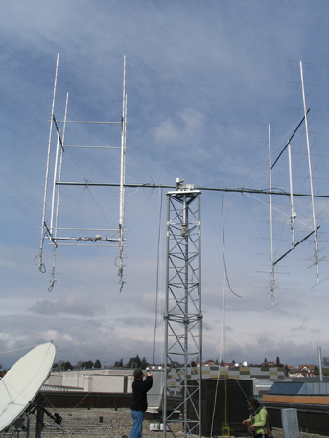
\includegraphics[width=0.32\paperwidth]{img/2/swisscube_groundstation.png}
            \caption{SwissCube EPFL ground station antennas. Source: \cite{swisscube_groundstation}}
            \label{PW-swisscube_groundstation}
        \end{figure}
    \end{minipage}
\end{minipage}